%% Cyberinfrastructure Shell (CIShell) Core Specification
%%
%% Copyright 2006,2007,2008 Indiana University
%%
%% Licensed under the Apache License, Version 2.0 (the "License");
%% you may not use this file except in compliance with the License.
%% You may obtain a copy of the License at
%%
%%     http://www.apache.org/licenses/LICENSE-2.0
%%
%% Unless required by applicable law or agreed to in writing, software
%% distributed under the License is distributed on an "AS IS" BASIS,
%% WITHOUT WARRANTIES OR CONDITIONS OF ANY KIND, either express or implied.
%% See the License for the specific language governing permissions and
%% limitations under the License.
%%
%

\chapter{GUI Builder Service Specification}
\section*{\textit{Version 1.0}}
\section{Introduction}

The GUI Builder Service provides a user-interface-agnostic solution to create UIs
for simple user input. The UIs are built from the user interface specification
provided by \class{MetaTypeProvider} and requires no UI coding to be done other
than providing an implementation of \class{MetaTypeProvider}. Information on
creating these classes can be found in section \ref{GUISpec}. In addition, simple
methods for creating warnings, pop-ups, and simple yes/no dialog boxes are
provided by the GUI Builder Service. The GUI creation workflow is illustrated in
figure \ref{fig:guiCreationWorkflow}.

\subsection{Entities}

\begin{itemize}
  \item \textit{GUIBuilderService} - The Service interface for creating
  user interfaces and dialog boxes.
  \item \textit{MetaTypeProvider} - The interface for creating simple user
  interface specifications.
  \item \textit{GUI} - The interface for controlling the
  \class{GUIBuilderService} generated user interface.
  \item \textit{SelectionListener} - The interface to listen for events
  generated by the user's interaction with the UI.
\end{itemize}

\begin{figure}[htb!]
\centering
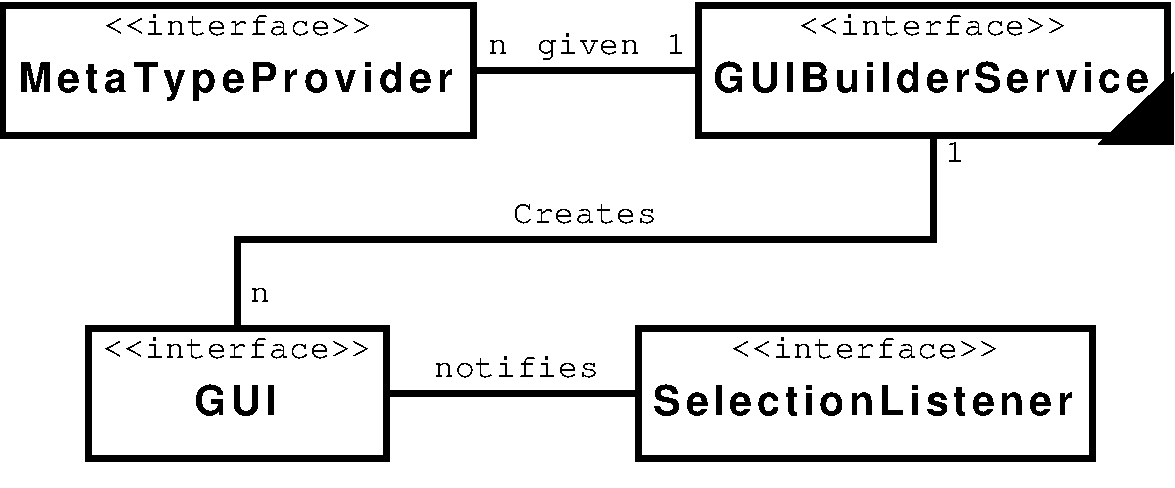
\includegraphics[width=90mm]{../img/guiCreationWorkflow.pdf}
\caption{GUI Creation Workflow}
\label{fig:guiCreationWorkflow}
\end{figure}

\orgcishellserviceguibuilder{}
